\chapter{Implementation}
In this section we will discuss the implementation of our previously discussed design. More specifically, the electronic hardware and software systems.

\section{Hardware implementation}
The hardware systems are implemented using two printed circuit boards (PCBs), one for each microcontroller. These handle the communication between the microcontrollers and the execution of actions, requested by the control device laptop.

\subsection{Printed Circuit Boards}

The first PCB is for the PIC18F slave microcontroller. The PIC18F resides in the middle and is the central unit of this board. The PCB contains a connection for the solenoid, to control when it need to turn on and off. It also contains connections for the servo motor and its control circuit which is a simple MOSFET transistor circuit. The board has connections for the NRF24 module, to make radio communication with the ESP32 possible. This PCB design can be seen in Figure~\ref{fig:pic-pcb}.

\begin{figure}[h]
	\centering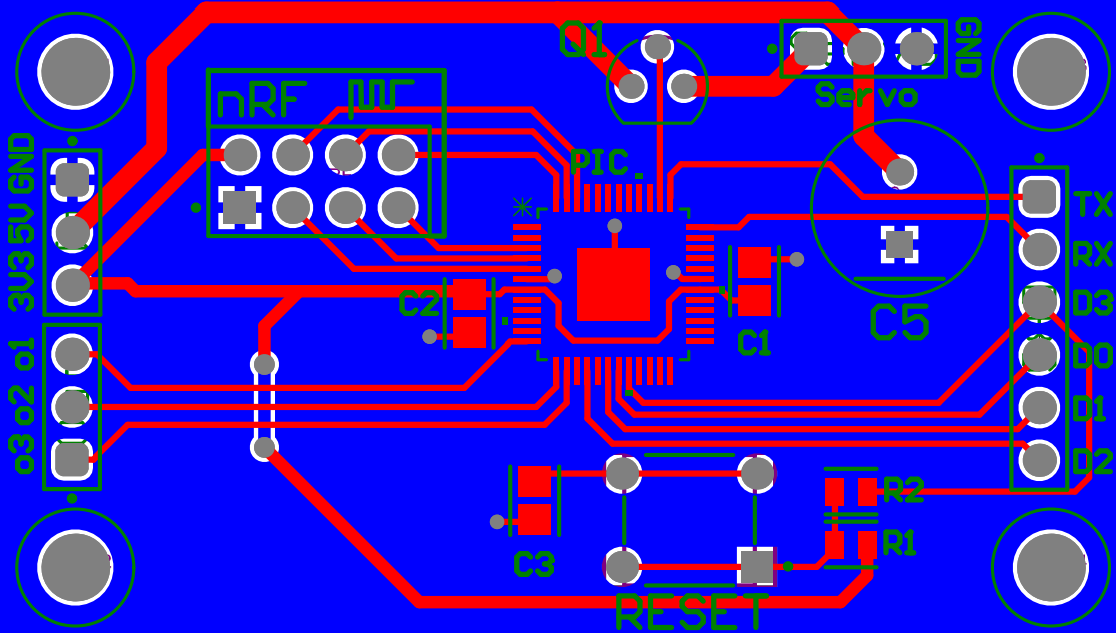
\includegraphics[height=5cm]{./images/PIC18F_pcb}
	\caption{PIC18F PCB Design}
	\label{fig:pic-pcb}
\end{figure}

The second PCB is for the ESP32 master controller. This PCB consists of pin headers for the ESP32 controller itself, and pin headers for each of the DRV8825 modules, which control the stepper motors. It has switches for on board adjustment of the drivers' control pins. It also contains connections for the NRF24 module, like the PIC18F. This PCB design can be seen in Figure~\ref{fig:esp-pcb}. 

\begin{figure}[h]
	\centering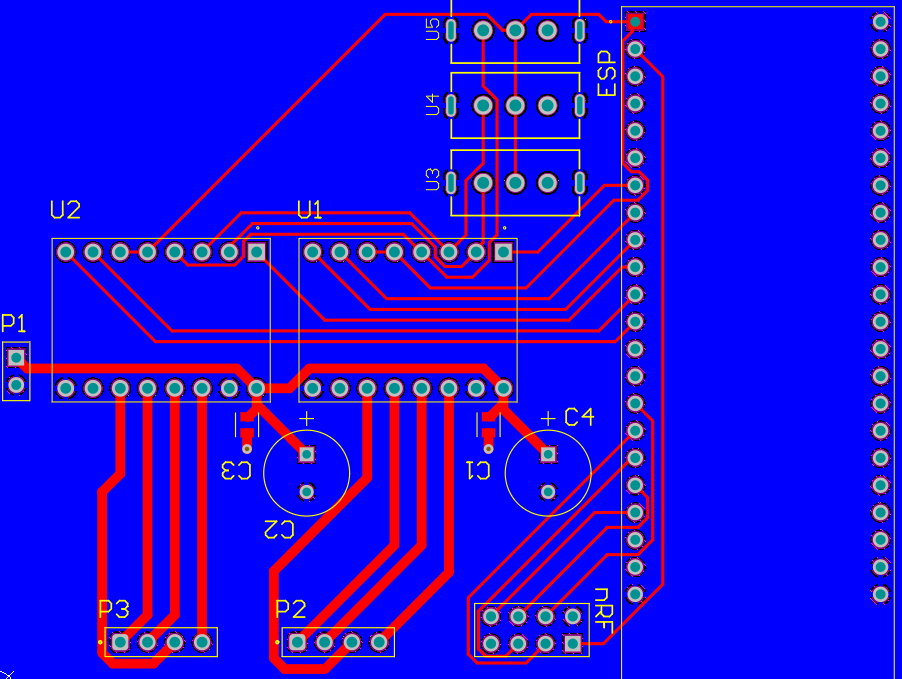
\includegraphics[height=5cm]{./images/ESP32_pcb}
	\caption{ESP32 PCB Design}
	\label{fig:esp-pcb}
\end{figure}


\section{Software implementation}

There are 3 main pieces of software for the proposed system. First, an ESP32 software suite for gantry control, networked communication, and radio communication. Secondly, the PIC18F software system which implements hardware control and radio communication. Finally, the final set of software is the desktop application for image tracking, communication, and sending control commands over the network.

\subsection{ESP32}
The ESP32 software is divided into a few important subsystems. The communication driver, which defines a User Datagram Protocol (UDP) controller loop. This receives dynamic instructions in a pre-specified format to control the gantry's position and the racket module. This system is modular and robust, allowing the user to rapidly prototype by adjusting only their command producer, while the ESP32 doesn't need reprogramming. The system is built on FreeRTOS with modular task division for consistent concurrent processing. These subsystems interact through well-defined interfaces and communicate via FreeRTOS message queues, allowing asynchronous data exchange and decoupling between components.

The overall system design reflects a deliberate emphasis on separation of concerns, real-time responsiveness, scalability, and testability. The modular task-based architecture and asynchronous queue-based messaging enable the system to maintain predictable real-time behavior while remaining adaptable to future expansions or modifications. The inclusion of simulation capabilities addresses the need for verification and debugging in complex embedded systems where hardware access may be limited during certain development phases.

The firmware includes compile-time configuration flags to enable or disable subsystems such as UDP communication, radio communication, stepper control, and mock simulation tasks. This configurability allows the firmware to be adapted for various development and deployment scenarios, including partial module testing, hardware-in-the-loop simulations, or full production operation.

\subsubsection{Communication Subsystem}
The communication subsystem is responsible for receiving external control commands via UDP over Wi-Fi and transmitting actuator signals through the NRF24 radio interface. The UDP client manages socket creation, data reception, and error handling, converting received commands into structured messages. These messages are placed into dedicated queues for consumption by the motion and actuator controllers. The NRF24-based radio communication provides an additional, low-latency communication channel for controlling remote actuators, contributing to the system's flexibility and scalability.

\subsubsection{Motion Control Subsystem}
The motion control subsystem handles the operation of two stepper motors along orthogonal axes. Motor control is implemented using hardware timers, configured to trigger interrupts at precise intervals. Within the interrupt service routines, step signals are toggled, positions are updated, and step frequencies are adjusted according to desired momentum and target positions. The use of easing functions ensures smooth acceleration and deceleration, minimizing mechanical stress and enabling precise control. Position and speed adjustments are driven by messages, received from the communication subsystem, allowing dynamic and responsive actuation.

\subsubsection{Simulation and Testing Subsystem}
To facilitate development and validation in the absence of hardware, the system incorporates a simulation and testing subsystem. Mock tasks generate synthetic messages simulating both UDP communication and actuator commands. This feature enables rigorous testing of system behavior, ensuring robustness and correctness prior to hardware deployment.

\subsubsection{Inter-task Communication and Decoupling}
The system employs three dedicated message queues for horizontal stepper control, vertical stepper control, and racket actuator commands. These queues enable asynchronous, thread-safe communication between tasks. The use of structured message formats for stepper and actuator commands maintains consistency and simplifies message handling logic, supporting scalability and modular expansion.

\subsection{Desktop}
The bulk of the application resides on a desktop environment. The desktop is connected to the same network as the IP cameras and the ESP32, this allows constant networked communication between these systems. The desktop application receives data constantly from the IP cameras. This data is then passed through an OpenCV image processing algorithm, developed to track and derive the 3D position of the ball in real time. The system implements a generic visualizer system which shows the ball position in real time along with a visual of the ping pong table. Finally, this data is all processed and passed to a GUI application, through which the user interfaces with the gantry. The system allows for automated and manual control via a set of buttons and sliders in the developed application.

\subsubsection{Ball Tracking}
An external computer vision module, in Python, implements a real-time system for tracking a ping-pong ball in 3D space using two phone cameras. It calibrates the cameras either automatically or manually by first, creating a projection matrix for the table through homography. This allows the system to map points from the camera’s 2D image onto the real-world plane of the table, effectively calibrating the table’s position in space. To further determine each camera’s exact location and orientation relative to the table, it uses a Perspective-n-Point (PnP) algorithm, which calculates the camera's position from known 3D–2D point correspondences. Once both cameras are calibrated, the system tracks the ball’s position in each 2D image using color filtering (in HSV color space) and circle detection, then computes the 3D location by finding the closest point between the two rays projected from each camera through the detected 2D ball positions.

\subsubsection{Network Communication}
The IP cameras are connected via the Hypertext Transfer Protocol (HTTP) to an OpenCV VideoCapture handle, which then applies the aforementioned ball tracking software. It then determines the gantry's target position, orientation, and firing state. This information is packaged into predefined data classes, which can be converted into a binary format that is interpretable by the target microcontroller. This information is then sent via a UDP connection, asynchronously, whenever a new input state is desired.

\subsubsection{Visualization}
Using matplotlib, a visualizer was implemented which can receive ball positions over an asynchronous queue, and visualize them in real time, this system is modular and easy to plug into other scripts.

\subsection{PIC18F}
The final software system implemented is the embedded controller on the PIC18F, this system constantly receives commands over the NRF24 module, which it then applies to its outputs. These commands include what angle to position a servo motor at, and when to "fire" the solenoid racket.


